\documentclass[12pt]{article}
\usepackage[left=0.25cm,top=1cm,right=0.25cm,bottom=1cm]{geometry}
\textwidth = 20cm
\hoffset = -1cm
\usepackage[utf8]{inputenc}
\usepackage[spanish,es-tabla]{babel}
\usepackage[autostyle,spanish=mexican]{csquotes}
\usepackage[tbtags]{amsmath}
\usepackage{nccmath}
\usepackage{amsthm}
\usepackage{amssymb}
\usepackage{graphicx}
\usepackage{standalone}
\usepackage[outdir=./]{epstopdf}
\usepackage{siunitx}
\usepackage{physics}
\usepackage{color}
\usepackage{float}
\usepackage{multicol}
%\usepackage{milista}
\usepackage{enumitem}
\usepackage{anyfontsize}
\usepackage{anysize}
\usepackage{enumitem}
\usepackage{capt-of}
\usepackage{bm}
\usepackage{relsize}
\usepackage{placeins}
\usepackage{empheq}
\usepackage{cancel}
\usepackage{wrapfig}
\spanishdecimal{.}
\renewcommand{\baselinestretch}{1.5} 
\renewcommand\labelenumii{\theenumi.{\arabic{enumii}}}
\newcommand{\ptilde}[1]{\ensuremath{{#1}^{\prime}}}
\newcommand{\stilde}[1]{\ensuremath{{#1}^{\prime \prime}}}
\newcommand{\ttilde}[1]{\ensuremath{{#1}^{\prime \prime \prime}}}
\newcommand{\ntilde}[2]{\ensuremath{{#1}^{(#2)}}}


\title{Tema 1 - Lista de ejercicios a cuenta\\ \large{Matemáticas Avanzadas de la Física}\vspace{-3ex}}
\author{M. en C. Gustavo Contreras Mayén}
\date{ }
\begin{document}
\vspace{-4cm}
\maketitle
\fontsize{14}{14}\selectfont
\section{Presentación 1}
\begin{enumerate}
\item Considera la transformación de coordenadas:
\begin{align*}
x &= 2 \, u \, v \\[0.5em]
y &= u^{2} + v^{2} \\[0.5em]
z &= w
\end{align*}
Demuestra que el nuevo sistema de coordenadas \emph{no} es ortogonal.
\end{enumerate}
\section{Presentación 2}
\begin{enumerate}
\item La velocidad y la aceleración se definen en la forma vectorial como:
\begin{align*}
\vb{v} = \dv{\vb{r}}{t} = \dot{\vb{r}} \hspace{1cm} \vb{a} = \dot{\vb{v}} = \ddot{\vb{r}}
\end{align*}
Calcula para el sistema coordenado esférico:
\begin{enumerate}
\item $\dot{\vu{e}}_{r}$, $\dot{\vu{e}}_{\theta}$, $\dot{\vu{e}}_{\varphi}$ 
\item La velocidad $\vb{v}$
\item La aceleración $\vb{a}$
\end{enumerate}
\pagebreak
\item Demuestra que para dos vectores $\vb{A}$ y $\vb{B}$:
\begin{enumerate}
\item $\vb{A} \cp \vb{B} = \displaystyle \sum_{ijk} \, \vu{e}_{i} \, \epsilon_{ijk} \, A_{j} \, B_{k}$
\item $\vb{A} \cdot \vb{B} \cp \vb{C} = \displaystyle \sum_{ijk} \, \epsilon_{ijk} \, A_{i} \, B_{j} \, C_{k}$
\end{enumerate}
\item Para ejercitar el avance que llevamos, resuelve:
\begin{enumerate}
\item Demuestra que $\grad{\phi \psi} = \phi \, \grad{\psi} + \psi \, \grad{\phi}$
\item Si $f = f(r)$ con $r = \sqrt{x^{2} + y^{2}+ z^{2}}$, demuestra que
\begin{align*}
\nabla{f(r)} = \vu{r} \, \dv{f(r)}{r}
\end{align*}
\end{enumerate}
\item Demuestra que el campo eléctrico de una carga puntal
\begin{align*}
\vb{E} = \dfrac{q \, \vu{r}}{4 \, \pi \epsilon_{0} \, r^{2}}
\end{align*}
cumple $\div{E} = 0$, para $r \neq 0$.
\item La ley de Gauss para el campo eléctrico tiene la forma:
\begin{align*}
\oint \vb{E} \cdot \dd{\vb{S}} = \dfrac{q}{\epsilon_{0}}
\end{align*}
donde $q = \displaystyle \int \rho \dd{V}$ es la carga encerrada en la superficie y $\rho$ su densidad volumétrica.
\\
\bigskip
Demuestra la ley de Gauss en forma diferencial
\begin{align*}
\div{E} = \dfrac{\rho}{\epsilon_{0}}
\end{align*}
\item Demuestra que:
\begin{align*}
\curl(\phi \, \vb{A}) = \phi \, \curl{\vb{A}} + \grad{\phi} \times \vb{A}
\end{align*}
\item El campo electrostático de un dipolo eléctrico $\vb{p} = p_{0} \, \vu{e}_{z}$ es
\begin{align*}
\vb{E} = \dfrac{p_{0} (2 \, \vb{e}_{r} \, \cos \theta + \vu{e}_{\theta} \, \sin \theta)}{r^{3}}
\end{align*}
Demuestra que:
\begin{enumerate}
\item $\curl{\vb{E}} = 0$
\item para $r \neq 0$, se tiene $\div{\vb{E}} = 0$
\end{enumerate}
\item Demuestra que el Laplaciano en coordenadas cilíndricas y esféricas es el que se presenta, para ello tendrás que calcular los respectivos factores de escala.
\end{enumerate}
\section{Presentación 3}
\begin{enumerate}
\item  Para el sistema de coordenadas esferoidales prolatas $(u, v, \varphi)$, cuyas reglas de transformación son:
\begin{align*}
x &= a \, \sinh u \, \sin v \, \cos \varphi \\
y &= a \, \sinh u \, \sin v \, \sin \varphi \\
z &= a \, \cosh u \, \cos v
\end{align*}
\begin{enumerate}
\item Describe las superficies coordenadas del sistema.
\item Calcula de manera explícita los factores de escala $(h_{u}, h_{v}, h_{\varphi})$.
\end{enumerate}
\item Ocupando el mismo el sistema de coordenadas esferoidales prolatas $(u, v, \varphi)$ del ejercicio a cuenta anterior: Calcula los operadores diferenciales $\grad{\phi}$, $\div{\vb{B}}$, $\curl{\vb{B}}$ y $\laplacian{\phi}$
\end{enumerate}
\section{Presentación 4.}
\begin{enumerate}
\item En una distribución tipo Maxwell la fracción de partículas moviéndose con velocidad $v$ y $v +\dd{v}$ es
\begin{align*}
\dfrac{\dd{N}}{N} = 4 \, \pi \left( \dfrac{m}{2 \, \pi \, k \, T} \right)^{3/2} \: \exp \left( - \dfrac{m \, v^{2}}{2 \, k \, T} \right) \: v^{2} \dd{v}
\end{align*}
donde $N$ es el número total de partículas. 
\par
El promedio o valor esperado de $v^{n}$ se define como $\displaystyle \expval{v^{n}} = N^{-1} \int v^{n} \dd{N}$.
\par
Demostrar que:
\begin{align*}
\expval{v^{n}} = \left( \dfrac{2 \, k \, T}{m} \right)^{n/2} \dfrac{\left( \dfrac{n + 1}{2} \right) !} { \left( \dfrac{1}{2} \right) !}
\end{align*}
\item Se muestra en la figura (\ref{fig:figura_cicloide}) parte de una cicloide cuyas ecuaciones paramétricas son
\begin{align*}
x &= a (\theta + \sin \theta) \\[0.5em]
y &= a (1 - \cos \theta)
\end{align*}
\begin{figure}[H]
        \centering
        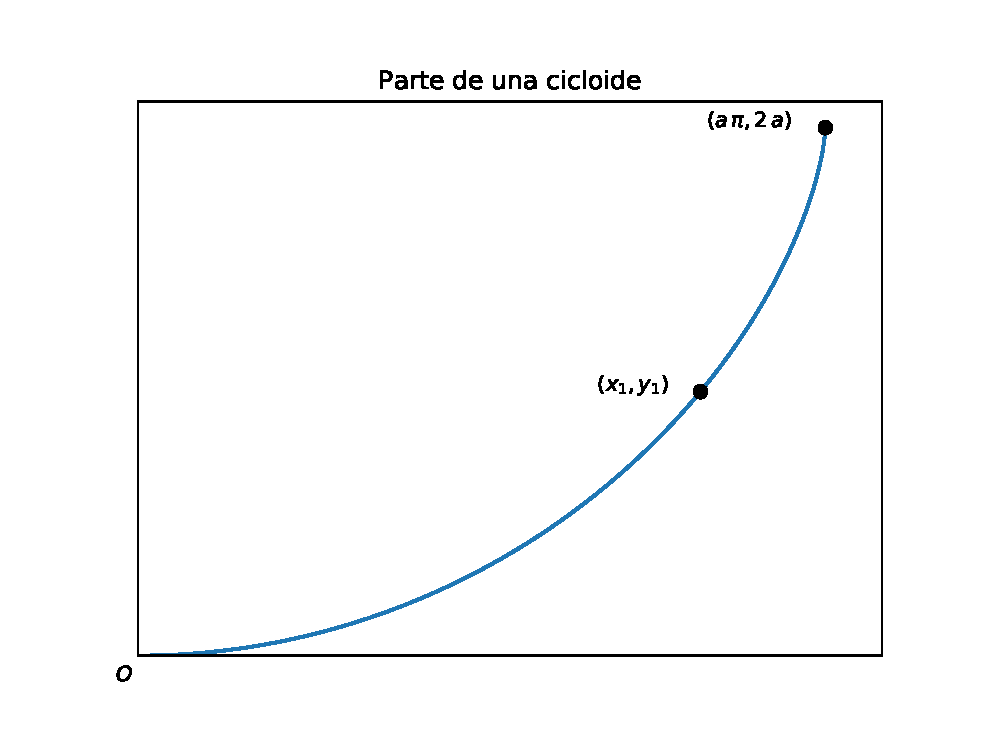
\includegraphics[width=0.5\textwidth]{Imagenes/plot_cicloide.eps}
        \caption{Una partícula deslizándose sobre una cicloide.}
        \label{fig:figura_cicloide}
\end{figure}
Demuestra que el tiempo que tarda una partícula para deslizarse sin fricción a lo largo de la curva desde el punto $(x_{1}, y_{1})$ hasta el origen, está dado por
\begin{align*}
t = \sqrt{\dfrac{a}{g}} \, \int_{0}^{y_{1}} \dfrac{\dd{y}}{\sqrt{y \, (y_{1}- y)}}
\end{align*}
Sugerencia: Demuestra que la longitud del elemento de arco es $\dd{s} = \sqrt{2a/y} \dd{y}$. Evalúa la integral para demostrar que el tiempo es independiente de la posición inicial $y_{1}$.
\end{enumerate}
\end{document}